% ── SLIDE 1: Motivation and question ──────────────────────────────────────────
\begin{frame}{Why hard carbon, and why pyrolysis conditions}
  \begin{itemize}
    \item Na-ion batteries avoid Li, Co and Ni --- but graphite does not intercalate
          \(\mathrm{Na^+}\). \textbf{Hard carbon} is the practical anode.
    \item Capacity and first-cycle losses are set by the \textbf{disordered microstructure}:
          closed pore volume, interlayer spacing, defect and surface-group density.
    \item That microstructure is controlled by how the biochar is pyrolysed ---
          \textbf{final temperature} and \textbf{heating ramp rate}.
    \item Ramp rate is far less studied than temperature, yet it plausibly governs
          how pores close and how volatiles escape.
  \end{itemize}
  \vspace{0.4em}
  \begin{block}{Research question}
    \small
    How do pyrolysis temperature (600--1200\,\({^\circ}\)C) and heating ramp rate
    (1--3\,\({^\circ}\)C/min at 1200\,\({^\circ}\)C) affect the electrochemical
    performance of MMB1 biochar hard carbon in Na half cells?
  \end{block}
  \note{Frame the material choice first: sodium is cheap and geopolitically safe, but
  graphite simply does not work, so the anode is the bottleneck and hard carbon is the
  candidate. The key idea is that hard carbon is not one material --- its performance is
  a direct function of how it was made. Temperature is well covered in the literature;
  ramp rate is not, which is where this project can contribute something new. Note that
  the ramp series is deliberately all at 1200 degrees so temperature is held constant
  and only the ramp varies.}
\end{frame}

% ── SLIDE 2: Samples and cells ────────────────────────────────────────────────
\begin{frame}{Samples, cells and test protocol}
  \begin{columns}[T]
    \begin{column}{0.54\textwidth}
      \begin{itemize}
        \item 6 MMB1 samples, N\(_2\), 2\,h hold
        \item \textbf{23 Na half cells}, CC19--CC41
        \item Kuranode commercial hard carbon as
              \textbf{benchmark control}
        \item Capacities normalised on the
              \textbf{measured} mass basis
              (5.5255\,mg foil tare + per-sample \(f\)),
              not the cycler's 5.55\,mg assumption
      \end{itemize}
      \vspace{0.3em}
      {\footnotesize
      \textbf{Protocol differs by instrument:}\\
      Bio-Logic C/10 to 2.2\,V\quad$\vert$\quad Neware C/20 to 2.0\,V}
    \end{column}
    \begin{column}{0.43\textwidth}
      \begin{table}
        \centering
        \footnotesize
        \begin{tabular}{@{}llc@{}}
          \toprule
          \textbf{Sample} & \textbf{Condition} & \textbf{Cells} \\
          \midrule
          MMB1\_6A  & 600\,\({^\circ}\)C, 3\,\({^\circ}\)C/min  & 2 \\
          MMB1\_8A  & 800\,\({^\circ}\)C, 3\,\({^\circ}\)C/min  & 1 \\
          MMB1\_10A & 1000\,\({^\circ}\)C, 3\,\({^\circ}\)C/min & 2 \\
          MMB1\_12A & 1200\,\({^\circ}\)C, 1\,\({^\circ}\)C/min & 5 \\
          MMB1\_12A & 1200\,\({^\circ}\)C, 2\,\({^\circ}\)C/min & 5 \\
          MMB1\_12A & 1200\,\({^\circ}\)C, 3\,\({^\circ}\)C/min & 5 \\
          Kuranode  & commercial ref.            & 2 \\
          \bottomrule
        \end{tabular}
        \caption{Cell build across the sample matrix.}\label{tab:matrix}
      \end{table}
    \end{column}
  \end{columns}
  \note{Stress two things here. First, the 1200 degree standard ramp of 3 degrees per
  minute plays a double role --- it is both the 1200 point of the temperature series and
  the 3 degree member of the ramp series, so 600, 800 and 1000 were all run at that same
  ramp. Second, the mass basis matters: the cycler assumed a fixed 5.55 mg and 91 percent
  active, and using the measured disk masses instead shifts every specific capacity. The
  two instruments used different rates and cutoffs, which is why they are never pooled
  without saying so.}
\end{frame}

% ── SLIDE 3: Data quality — what is usable ────────────────────────────────────
\begin{frame}{Not all 23 cells are usable}
  \begin{columns}[T]
    \begin{column}{0.55\textwidth}
      \begin{table}
        \centering
        \scriptsize
        \begin{tabular}{@{}lll@{}}
          \toprule
          \textbf{Cell} & \textbf{Failure} & \textbf{Evidence} \\
          \midrule
          CC31 & no data      & 67 pts, negative Re(\(Z\)) \\
          CC30 & failed coating & 0.561\,mg active; CE 88--96\,\% \\
          CC27 & soft short   & \(\vert Z\vert\) 79\,\(\Omega\) vs 700--2500 \\
          CC24 & bad contact  & jumpy onset \(V\); ICE 59\,\% \\
          CC41 & no local export & re-pull from server \\
          \bottomrule
        \end{tabular}
        \caption{Five excluded cells --- five distinct causes.}\label{tab:bad}
      \end{table}
    \end{column}
    \begin{column}{0.42\textwidth}
      \begin{itemize}
        \item \textbf{800\,\({^\circ}\)C lost entirely} --- its only cell was
              a failed coating
        \item \textbf{600\,\({^\circ}\)C unreplicated} --- CC31 died at assembly
        \item \textbf{Ramp series intact}: 3--4 cells per group
      \end{itemize}
    \end{column}
  \end{columns}
  \vspace{-0.2em}
  \begin{block}{}
    \footnotesize
    Five failures, five unrelated causes --- so there is \textbf{no single process fault}
    to correct. The temperature series is the casualty; the ramp series survives.
  \end{block}
  \note{Do not skip this slide --- it is what makes everything after it credible. The
  important point is the diversity of causes: if all five had failed the same way it would
  point at one bad step in the build, but they did not. CC30 is the expensive one because
  it removes the entire 800 degree condition, and CC31 leaves 600 with a single
  unconfirmable cell. Fortunately the ramp rate comparison, which is the actual research
  question, is untouched and has three to four cells per group.}
\end{frame}

% ── SLIDE 4: ICE — the solid result ───────────────────────────────────────────
\begin{frame}{Initial coulombic efficiency rises with temperature}
  \begin{columns}[T]
    \begin{column}{0.40\textwidth}
      \begin{itemize}
        \item ICE \(=\) desodiation\(_1\) / sodiation\(_1\)
        \item Measured in \textbf{cycle 1}, before any of the
              degradation discussed later
        \item \textbf{Temperature:} 34\,\% \(\rightarrow\) 60\,\%
              \(\rightarrow\) 66\,\% --- the expected direction, as
              higher pyrolysis removes defects and surface groups
              that trap Na irreversibly
        \item \textbf{Ramp rate: flat} (71 / 71 / 66\,\%)
      \end{itemize}
      \vspace{0.2em}
      {\scriptsize \textbf{Temperature drives ICE, not ramp rate.}}
    \end{column}
    \begin{column}{0.57\textwidth}
      \begin{figure}
        \centering
        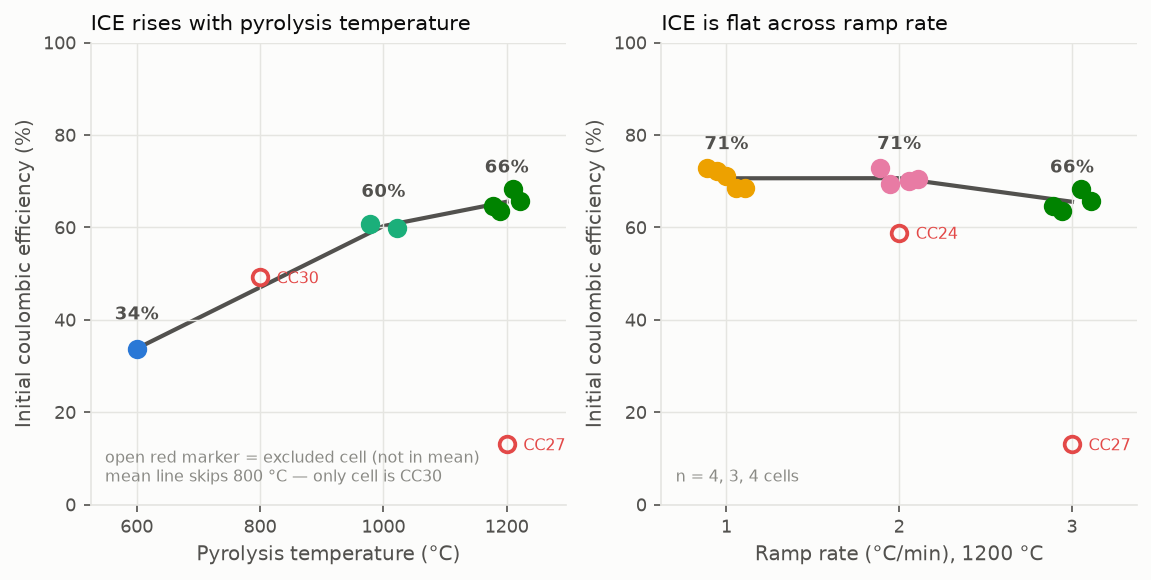
\includegraphics[width=\linewidth,height=0.70\textheight,keepaspectratio]{Figures/04_ICE_temperature_and_ramprate.png}
        \caption{ICE by temperature (left) and ramp rate (right); replicates jittered.}\label{fig:ice}
      \end{figure}
    \end{column}
  \end{columns}
  \note{This is the most defensible result in the dataset and that is why it comes first.
  ICE is measured entirely within cycle one, so it is immune to the fade artifact shown in
  two slides time. The physical story is standard and reassuring: higher pyrolysis
  temperature removes the defects and oxygen surface groups that consume sodium
  irreversibly into the SEI, so less charge is lost on the first sodiation. The contrast
  with the flat ramp rate response is itself informative --- it says ICE is set by final
  temperature, not by the path taken to get there. Flag that 600 and 800 are weak
  endpoints with n equals one.}
\end{frame}

% ── SLIDE 5: Ramp rate — the core question ────────────────────────────────────
\begin{frame}{Slower ramp gives higher capacity at 1200\,\({^\circ}\)C}
  \begin{columns}[T]
    \begin{column}{0.40\textwidth}
      \begin{itemize}
        \item All three groups: \textbf{same temperature, same
              electrode process}, 3--4 cells each
        \item \textbf{1\,\({^\circ}\)C/min sits clearly above}
              2 and 3\,\({^\circ}\)C/min across every cycle
        \item Replicate scatter is well separated between groups
        \item \textbf{The cleanest comparison in the dataset} ---
              and the project's actual question
      \end{itemize}
      \vspace{0.2em}
      {\scriptsize Slower heating plausibly allows more ordered
      pore closure.}
    \end{column}
    \begin{column}{0.57\textwidth}
      \begin{figure}
        \centering
        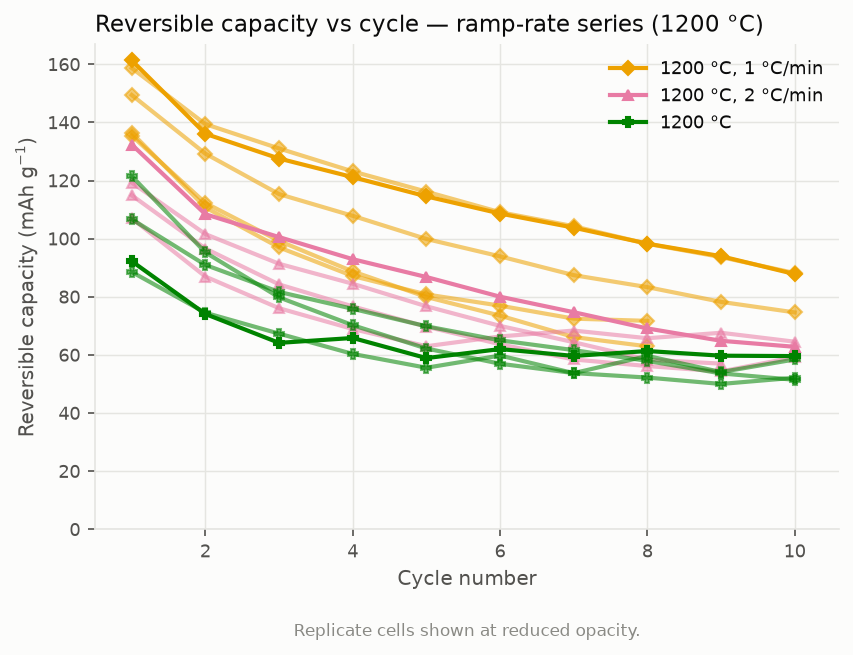
\includegraphics[width=\linewidth,height=0.70\textheight,keepaspectratio]{Figures/03_capacity_vs_cycle_ramprate.png}
        \caption{Reversible capacity vs cycle for the three 1200\,\({^\circ}\)C ramp rates.}\label{fig:ramp}
      \end{figure}
    \end{column}
  \end{columns}
  \note{This is the headline claim for the project. It is the cleanest comparison
  available because temperature is held fixed at 1200, the electrode processing is
  identical, and there are three to four cells in each group so the separation is not one
  lucky cell. Be honest that the mechanism is a hypothesis at this stage: slower heating
  should give volatiles more time to leave and pores more time to close in an ordered way,
  but that needs the XRD and Raman to confirm. Also be clear that this is the claim most
  worth re-confirming once the degradation issue on the next slide is fixed.}
\end{frame}

% ── SLIDE 6: The fade problem ─────────────────────────────────────────────────
\begin{frame}{A systemic fade affects every cell --- including the control}
  \begin{columns}[T]
    \begin{column}{0.40\textwidth}
      \begin{itemize}\footnotesize
        \item Every cell loses \textbf{35--45\,\%} of reversible
              capacity over 10 cycles --- at \textbf{CE \(\approx\) 100\,\%}
        \item Near-perfect CE with steady fade means Na is not being
              consumed; \textbf{less material is participating}
        \item The \textbf{Kuranode commercial benchmark} (heavy line)
              fades as fast as or faster than the biochar
      \end{itemize}
      \vspace{0.3em}
      \begin{block}{}
        \scriptsize
        A control that fails like the samples means the fade is
        \textbf{cell-build / test-side}, not a property of the material.
        \textbf{Retention is therefore not reported as a result.}
      \end{block}
    \end{column}
    \begin{column}{0.57\textwidth}
      \begin{figure}
        \centering
        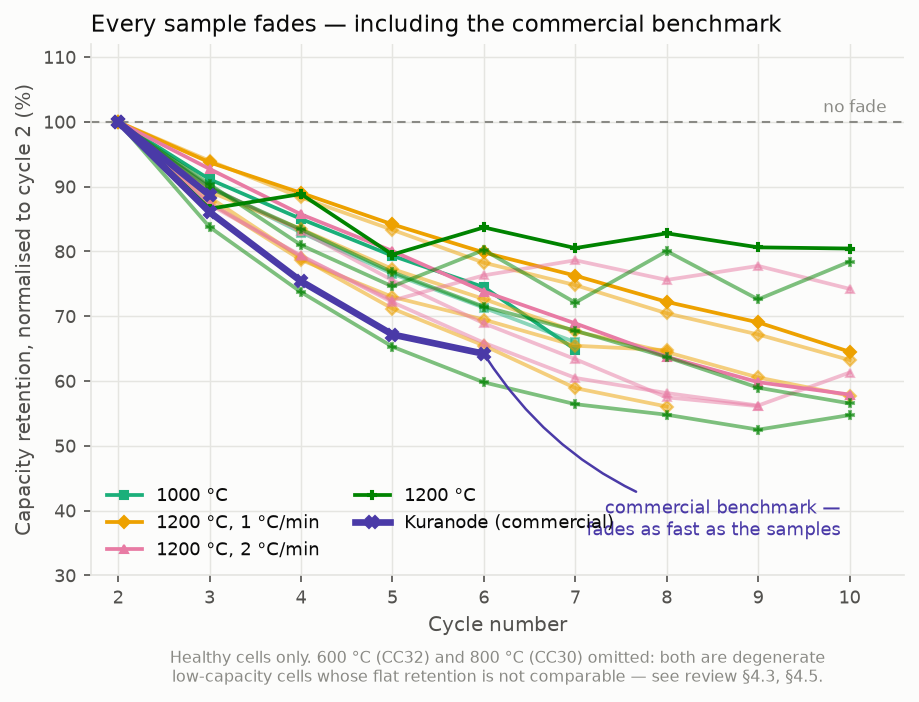
\includegraphics[width=\linewidth,height=0.70\textheight,keepaspectratio]{Figures/01_systemic_fade_all_samples.png}
        \caption{Capacity normalised to each cell's own cycle 2.}\label{fig:fade}
      \end{figure}
    \end{column}
  \end{columns}
  \note{Present this as a finding, not as an apology. The logic is what matters: the
  Kuranode is a commercial reference material that is known to cycle stably, so when it
  fades exactly like our biochar the fault cannot be in the biochar. Normalising every
  cell to its own cycle two removes the absolute capacity differences and compares only the
  shape of the decay. The coulombic efficiency detail is the strongest single clue --- if
  sodium were being consumed chemically the CE would drop below 100, and it does not, so
  something is progressively disconnecting rather than reacting. 600 and 800 are omitted
  because their degenerate low-capacity cells would falsely suggest stability.}
\end{frame}

% ── SLIDE 7: Impedance ruled out ──────────────────────────────────────────────
\begin{frame}{The obvious explanation was tested --- and rejected}
  \begin{columns}[T]
    \begin{column}{0.40\textwidth}
      \begin{itemize}\footnotesize
        \item \textbf{Hypothesis:} the fade is rising cell impedance
        \item \(\vert Z\vert\) at 1\,Hz recovered from the raw
              \texttt{.mpr} binaries at four stages
        \item \textbf{Result: impedance \emph{falls} 14--28\,\%} from
              post-formation to post-cycling, in every cell
        \item So the rising desodiation onset voltage is a
              \textbf{consequence} of less Na inserted, not a cause
      \end{itemize}
      \vspace{0.2em}
      {\scriptsize \textbf{Caveat:} two-electrode cells lump the carbon with the
      Na counter --- this excludes a gross whole-cell rise, not localised
      contact loss.}
    \end{column}
    \begin{column}{0.57\textwidth}
      \begin{figure}
        \centering
        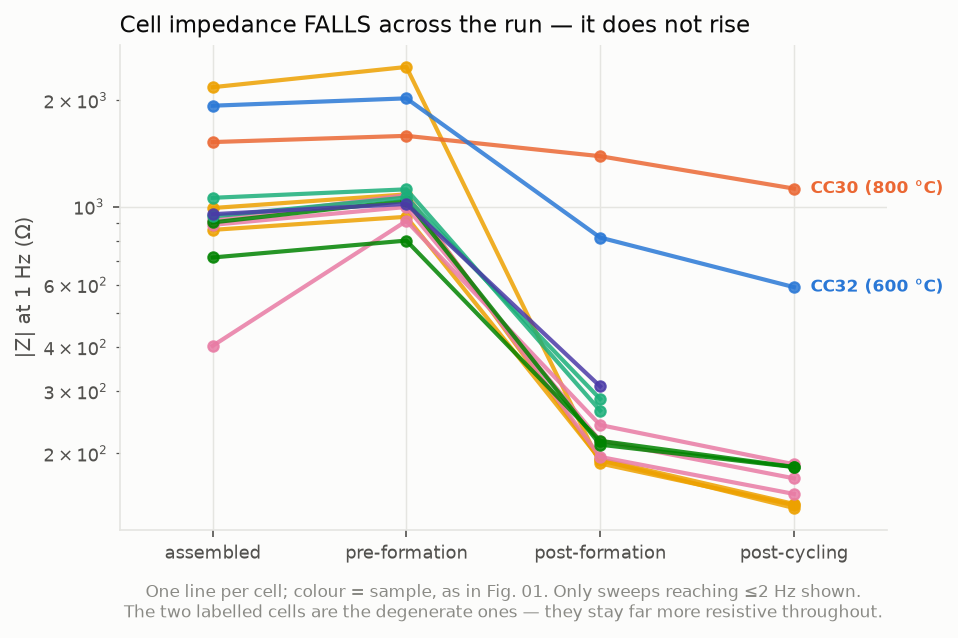
\includegraphics[width=\linewidth,height=0.70\textheight,keepaspectratio]{Figures/06_EIS_impedance_by_stage.png}
        \caption{\(\vert Z\vert\) at 1\,Hz by test stage, one line per cell (log axis).}\label{fig:eis}
      \end{figure}
    \end{column}
  \end{columns}
  \note{The point of this slide is to show the problem was investigated properly rather
  than just noted. Rising impedance is what everyone would guess first, and the EIS
  refutes it cleanly and in the same direction for every cell. Be scrupulous about the
  two-electrode caveat --- these are coin cells with no reference electrode, so the
  measurement lumps the working and counter electrodes together, and the large drop after
  formation is most likely the sodium surface activating. That could in principle mask a
  working-electrode process, so the honest statement is that a gross whole-cell impedance
  rise is excluded while localised contact loss is not. CC30 and CC32 stay four to eight
  times more resistive throughout, which independently confirms both are degenerate.}
\end{frame}

% ── SLIDE 8: Conclusions ──────────────────────────────────────────────────────
\begin{frame}{Conclusions}
  \begin{block}{What can be trusted now}
    \small
    \begin{itemize}
      \item \textbf{ICE rises strongly with pyrolysis temperature}
            (34 \(\rightarrow\) 60 \(\rightarrow\) 66\,\%) and is
            \textbf{flat across ramp rate} --- consistent on both instruments.
      \item \textbf{1\,\({^\circ}\)C/min outperforms 2 and 3\,\({^\circ}\)C/min}
            at 1200\,\({^\circ}\)C, with 3--4 replicates per group.
      \item 1000\,\({^\circ}\)C gives the highest capacity of the temperatures measured.
    \end{itemize}
  \end{block}
  \begin{block}{What must not be reported yet}
    \small
    \begin{itemize}
      \item \textbf{Capacity retention} --- a systemic, cell-build-side fade affects
            every cell including the commercial control.
      \item \textbf{800\,\({^\circ}\)C} --- no valid cell exists.
      \item Bio-Logic and Neware results \textbf{are not pooled}: different rate and cutoff.
    \end{itemize}
  \end{block}
  \note{Keep this crisp and resist the temptation to over-claim. The two positive results
  are genuinely solid and both rest on replicates. The retention point is the one to be
  firm about --- it would be easy to quote a retention number and it would be wrong,
  because the control fades too. Ending with a clear separation of what is trustworthy from
  what is pending is the honest position and it sets up the outlook slide.}
\end{frame}

% ── SLIDE 9: Future outlook ───────────────────────────────────────────────────
\begin{frame}{Future outlook --- next experiments}
  \begin{columns}[T]
    \begin{column}{0.49\textwidth}
      \begin{block}{New 8\,A slurry (highest priority)}
        \begin{itemize}\scriptsize
          \item CC30 gave \textbf{0.561\,mg} active --- the coating was
                \(\sim\)11\,\% of the foil tare
          \item CE never closed (88--96\,\%): leakage dominated a tiny signal
          \item \textbf{Re-do the MMB1\_8A slurry} and re-coat: check solids
                loading, dispersion time and blade gap
          \item Target the \(\sim\)12--20\,mg disk mass range of the
                successful 1200\,\({^\circ}\)C coatings
          \item Without it there is \textbf{no 800\,\({^\circ}\)C point} in the
                temperature series
        \end{itemize}
      \end{block}
    \end{column}
    \begin{column}{0.49\textwidth}
      \begin{block}{Recommended new cells}
        \begin{itemize}\scriptsize
          \item \textbf{8\,A \(\times\) 3} --- from the new slurry, rebuilds the
                800\,\({^\circ}\)C condition
          \item \textbf{6\,A \(\times\) 2} --- CC32 is currently unreplicated
                and unconfirmable
          \item \textbf{Kuranode \(\times\) 2, run long} --- 3 and 6 cycles is
                not enough for a benchmark
          \item \textbf{10\,A \(\times\) 1} --- extends 7 cycles to a full run
        \end{itemize}
      \end{block}
      \vspace{-0.3em}
      {\scriptsize \textbf{Order matters:} diagnose the fade \emph{first}
      (electrolyte volume, Na counter, adhesion, stack pressure) --- every cell
      built before that is fixed will repeat the artifact.}
    \end{column}
  \end{columns}
  \note{Lead with the 8A slurry because it is the only way to recover a whole missing
  condition, and it is a synthesis problem rather than a measurement problem so it can start
  immediately. The mass numbers make the case: 0.561 mg of active material against roughly
  twelve to twenty on the good cells is not a marginal coating, it is essentially bare foil.
  On the new cells, the sequencing point is the one to emphasise --- building eight more
  cells before diagnosing the fade would just produce eight more cells with the same
  artifact, so the diagnosis comes first even though it is less satisfying. Also mention
  disassembling CC27 and CC24 as cheap diagnostics, and re-pulling CC41 from the server.}
\end{frame}

% ── SLIDE 10: Backup ──────────────────────────────────────────────────────────
\begin{frame}[noframenumbering]{Backup --- temperature series and instrument cross-check}
  \begin{columns}[T]
    \begin{column}{0.49\textwidth}
      \begin{figure}
        \centering
        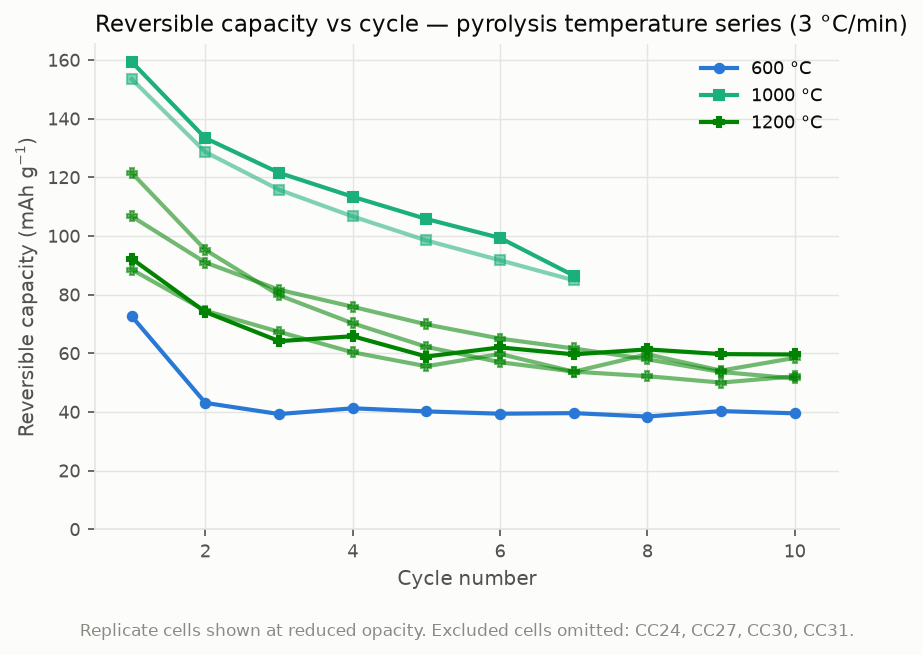
\includegraphics[width=\linewidth,height=0.60\textheight,keepaspectratio]{Figures/02_capacity_vs_cycle_temperature.png}
        \caption{Capacity vs cycle by pyrolysis temperature (800\,\({^\circ}\)C absent).}\label{fig:temp}
      \end{figure}
    \end{column}
    \begin{column}{0.49\textwidth}
      \begin{figure}
        \centering
        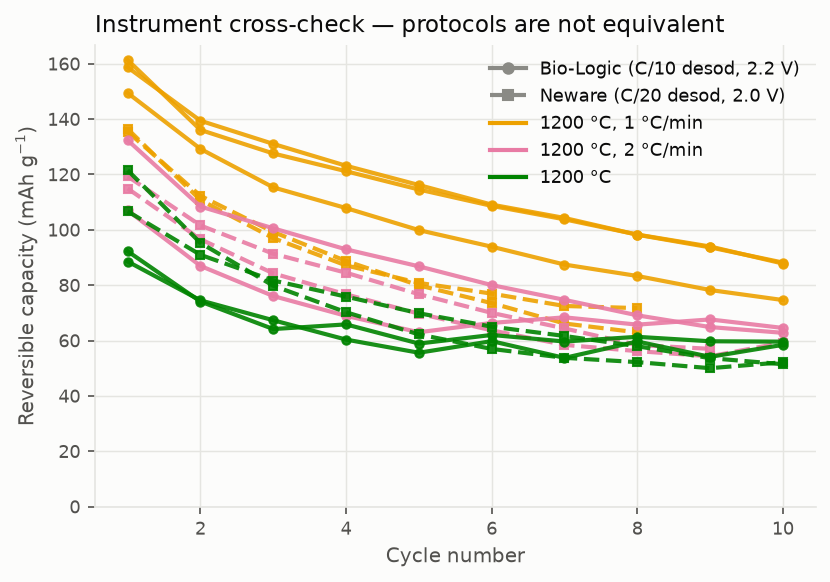
\includegraphics[width=\linewidth,height=0.60\textheight,keepaspectratio]{Figures/05_instrument_crosscheck.png}
        \caption{Bio-Logic (solid) vs Neware (dashed) on the same three samples.}\label{fig:cross}
      \end{figure}
    \end{column}
  \end{columns}
  \note{Backup slides. Use the left one if asked about absolute capacity by temperature ---
  1000 degrees is the highest performer, above 1200, but only cycles one and two should be
  read because later cycles carry the fade artifact. Use the right one if asked whether the
  two instruments can be combined: the answer is not directly, because Bio-Logic desodiates
  at C over 10 to 2.2 volts while Neware uses C over 20 to 2.0 volts, and Neware reads
  consistently lower.}
\end{frame}

% ── SLIDE 11: Backup — reading a single cell ──────────────────────────────────
\begin{frame}[noframenumbering]{Backup --- how to read a single cell}
  \begin{columns}[T]
    \begin{column}{0.45\textwidth}
      \begin{itemize}
        \item \textbf{Top:} sodiation (Na in, discharge) and desodiation
              (Na out, charge) per cycle
        \item The \textbf{gap} between them is Na not recovered
        \item \textbf{Bottom:} CE with a 100\,\% reference
        \item Reversible capacity is the \textbf{desodiation} value
      \end{itemize}
      \vspace{0.3em}
      {\scriptsize CC19: 221 in / 161 out on cycle 1 (ICE 72.9\,\%) --- SEI plus
      trapped Na. From cycle 2 the curves overlap at CE 99--100\,\%, yet
      capacity still falls.}
    \end{column}
    \begin{column}{0.52\textwidth}
      \begin{figure}
        \centering
        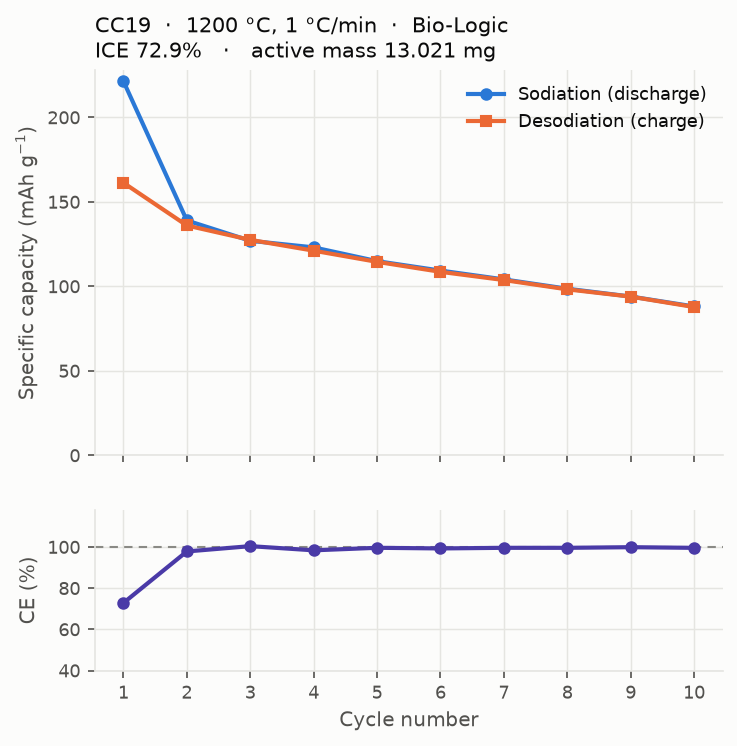
\includegraphics[width=\linewidth,height=0.70\textheight,keepaspectratio]{Figures/cells/CC19.png}
        \caption{CC19 --- a clean, well-behaved cell.}\label{fig:cc19}
      \end{figure}
    \end{column}
  \end{columns}
  \note{Use this if anyone asks how the raw per-cell data looks or why discharge equals
  sodiation. In a half cell the counter electrode is sodium metal, so discharging the cell
  spontaneously strips sodium from the metal and inserts it into the hard carbon --- that is
  sodiation. Note this inverts in a full cell, where the hard carbon is the anode and
  sodiates on charge, which is why both terms are always labelled. There are 21 of these,
  one per cell with data, and they are what the exclusion decisions were made from.}
\end{frame}

% ── SLIDE 12: References ──────────────────────────────────────────────────────
\begin{frame}{References}
  \footnotesize
  % TODO: add references — placeholders below, replace with the actual papers
  \begin{enumerate}
    \item % TODO
          Author \textit{et al.}, ``Hard carbon anodes for sodium-ion batteries,''
          \textit{Journal}, vol.~X, pp.~Y--Z, YEAR. doi:\texttt{10.XXXX/...}
    \item % TODO
          Author \textit{et al.}, ``Effect of pyrolysis temperature on hard carbon
          microstructure,'' \textit{Journal}, vol.~X, pp.~Y--Z, YEAR.
    \item % TODO
          Author \textit{et al.}, ``Closed porosity and the low-voltage plateau in
          hard carbon,'' \textit{Journal}, vol.~X, pp.~Y--Z, YEAR.
  \end{enumerate}
  \vspace{0.5em}
  {\scriptsize Full analysis, exclusions and data-quality findings:
  \texttt{Processes/Cycling\_Data\_Review\_2026-07-21.md}}
  \note{Keep this short. Point at the review document as the auditable record behind every
  number in the talk if anyone wants the detail.}
\end{frame}
